\documentclass[tikz]{standalone}
\usepackage{amsmath}
\usepackage{amssymb}
\usepackage{tikz}
\usepackage{xcolor}
\usepackage{bm}         % For bold math symbols
\usetikzlibrary{arrows.meta} % For better arrow tips

\begin{document}

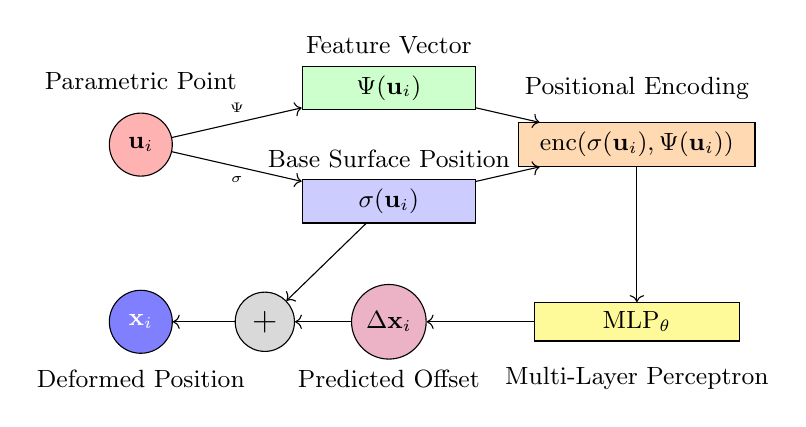
\begin{tikzpicture}[scale=0.9]

    % Sample point u_i
    \node[draw, circle, fill=red!30, minimum size=0.8cm] (u) at (0,0) {\small $\mathbf{u}_i$};
    \node at (0,0.9) {\small Parametric Point};

    % Psi(u)
    \node[draw, rectangle, fill=green!20, minimum width=2.2cm] (psi) at (3.5,0.8) {\small $\Psi(\mathbf{u}_i)$};
    \node at (3.5,1.4) {\small Feature Vector};

    % Sigma(u)
    \node[draw, rectangle, fill=blue!20, minimum width=2.2cm] (sigma) at (3.5,-0.8) {\small $\sigma(\mathbf{u}_i)$};
    \node at (3.5,-0.2) {\small Base Surface Position};

    % Encoding node
    \node[draw, rectangle, fill=orange!30, minimum width=3cm] (enc) at (7,0) {\small $\text{enc}(\sigma(\mathbf{u}_i), \Psi(\mathbf{u}_i))$};
    \node at (7,0.8) {\small Positional Encoding};

    % MLP node
    \node[draw, rectangle, fill=yellow!40, minimum width=2.6cm] (mlp) at (7,-2.5) {\small $\text{MLP}_\theta$};
    \node at (7,-3.3) {\small Multi-Layer Perceptron};

    % Displacement vector
    \node[draw, circle, fill=purple!30, minimum size=0.8cm] (dx) at (3.5,-2.5) {\small $\Delta \mathbf{x}_i$};
    \node at (3.5,-3.3) {\small Predicted Offset};

    % Plus node for summing sigma(ui) and delta_x (smaller + symbol)
    \node[draw, circle, fill=gray!30, minimum size=0.6cm] (plus) at (1.75,-2.5) {\large $+$};

    % Final position
    \node[draw, circle, fill=blue!50, text=white, minimum size=0.8cm] (x) at (0,-2.5) {\small $\mathbf{x}_i$};
    \node at (0,-3.3) {\small Deformed Position};

    % Arrows
    \draw[->] (u) -- (psi) node[midway, above] {\tiny $\Psi$};
    \draw[->] (u) -- (sigma) node[midway, below] {\tiny $\sigma$};
    \draw[->] (sigma) -- (enc);
    \draw[->] (psi) -- (enc);
    \draw[->] (enc) -- (mlp);
    \draw[->] (mlp) -- (dx);
    \draw[->] (sigma) -- (plus);
    \draw[->] (dx) -- (plus);
    \draw[->] (plus) -- (x);

  \end{tikzpicture}
\end{document}
